\documentclass[conference]{IEEEtran}
\IEEEoverridecommandlockouts
\usepackage{cite}
\usepackage{amsmath,amssymb,amsfonts}
\usepackage{graphicx}
\usepackage{textcomp}
\usepackage{xcolor}
\usepackage{array}
\def\BibTeX{{\rm B\kern-.05em{\sc i\kern-.025em b}\kern-.08em
    T\kern-.1667em\lower.7ex\hbox{E}\kern-.125emX}}

\begin{document}

\title{Multi-Model Boundary Refinement for Person Segmentation}

\author{
\IEEEauthorblockN{Final Project Team}
\IEEEauthorblockA{\textit{Artificial Intelligence Applications Course Project} \\
\textit{Course Final Report} \\
Taiwan}
}

\maketitle

\begin{abstract}
Person segmentation is useful in image editing, human-centered vision, and background removal tasks, but the final mask boundary is often unstable around hair, clothing, shadows, and complex backgrounds. This project studies a practical multi-model pipeline for improving person boundary segmentation without training a new neural network. The proposed workflow combines YOLO-based person localization, Segment Anything Model (SAM)-based mask generation, Canny edge detection for boundary checking, edge-based morphological refinement, and GrabCut foreground refinement. Eight experimental versions were prepared and six were batch-tested on twelve selected person images. The baseline version, automatic SAM with Canny scoring and GrabCut, achieved a mean edge alignment score of 0.8708. The proposed final version, YOLO-guided SAM with edge refinement and GrabCut, achieved the highest mean score of 0.8855, corresponding to a modest 0.0147 absolute improvement on the selected test set. The result suggests that using YOLO as an automatic box-prompt generator can reduce target ambiguity for SAM, while lightweight edge and foreground refinement can improve boundary stability. This project is a preliminary course-level study and uses edge alignment as a proxy metric because manually annotated ground-truth masks were not available.
\end{abstract}

\begin{IEEEkeywords}
person segmentation, Segment Anything Model, YOLOv8, Canny edge detection, GrabCut, boundary refinement
\end{IEEEkeywords}

\section{Introduction}
Person segmentation aims to separate the human subject from the background in an image. A segmentation mask may look acceptable at a rough object level, but small boundary errors can still make the result visually poor. This is especially clear around hair, arms, clothing edges, shadows, and backgrounds with similar colors. In this project, the main goal is not to design a new segmentation network, but to improve the practical boundary quality of person segmentation by combining several existing models and image-processing modules.

The initial direction of this project used edge maps to judge whether a generated person mask matched visible image boundaries. During the midterm review, the main feedback was that more models should be included and that the output precision was still insufficient. Based on that feedback, this final version expands the system into a multi-model comparison framework. SAM is used as the main segmentation module, YOLO is used for person localization and YOLO-Seg comparison, Canny edge detection is used for boundary scoring, and GrabCut is used as a lightweight foreground refinement step.

The main contributions of this project are:
\begin{itemize}
\item a complete multi-version pipeline for comparing SAM, YOLO-guided SAM, YOLO-Seg, Canny edge refinement, and GrabCut;
\item a simple edge alignment score for comparing boundary consistency when ground-truth masks are not available;
\item a preliminary experimental comparison on twelve selected person images from a larger set of uploaded test photos.
\end{itemize}

\section{Related Work}
\subsection{Promptable Segmentation}
The Segment Anything Model (SAM) introduced promptable segmentation, where a mask can be generated from prompts such as points, boxes, or existing masks \cite{kirillov2023segmentanything}. This makes SAM suitable for a course project because the model can be used directly without collecting a large training dataset. However, SAM output depends strongly on prompt quality. If the prompt is ambiguous or if automatic mask selection chooses the wrong region, the final mask may not correspond to the intended person.

Previous studies also show that prompt strategy affects SAM performance. Gaus et al. evaluated SAM with different prompting settings and showed that prompting design changes the segmentation result \cite{gaus2024variationalprompting}. Mazurowski et al. reported that box prompts can be more reliable than sparse point prompts in their experimental setting \cite{mazurowski2023sammedical}. These studies support the decision to use YOLO-detected person boxes as automatic prompts for SAM.

\subsection{YOLO Detection and Segmentation}
YOLO models are widely used for efficient object detection. A review of YOLO architectures describes the development from early YOLO versions to YOLOv8 and YOLO-NAS, showing why YOLO-based methods are common choices for real-time object localization \cite{terven2023yoloreview}. In this project, YOLOv8n is used to detect the person bounding box, and YOLOv8n-Seg is used as a direct segmentation comparison. The detection model provides a box prompt for SAM, while the segmentation model produces a mask directly.

\subsection{Classical Boundary Refinement}
Canny edge detection is a classical method for extracting structural image edges \cite{canny1986computational}. In this project, Canny edges are not treated as the final segmentation result. Instead, they are used as a boundary signal to judge whether the predicted mask boundary is close to visible image edges.

GrabCut is an interactive foreground extraction method based on iterated graph cuts \cite{rother2004grabcut}. It uses foreground and background information to refine object separation. This project uses the model-generated mask as an initialization for GrabCut, making it a lightweight post-processing module rather than an interactive tool.

\section{Methodology}
\subsection{System Overview}
The final system is organized as a modular pipeline. Each input image is processed by one of several version settings. Depending on the selected version, the image may pass through automatic SAM mask generation, YOLO person detection, YOLO-Seg mask generation, Canny edge-map generation, edge-based candidate refinement, and GrabCut refinement. Fig.~\ref{fig:pipeline} shows the strict system block diagram used to separate the baseline path, the proposed path, and the evaluation signal. Fig.~\ref{fig:progress} summarizes the dataset progress used for the final experiment.

\begin{figure*}[t]
\centering
\scriptsize
\setlength{\tabcolsep}{3pt}
\renewcommand{\arraystretch}{1.25}
\begin{tabular}{c c c c c c c c c}
\fbox{\begin{minipage}[c][0.55in][c]{0.95in}\centering\textbf{Input}\\person photo\end{minipage}}
& $\rightarrow$ &
\fbox{\begin{minipage}[c][0.55in][c]{1.05in}\centering\textbf{YOLOv8n}\\person box\end{minipage}}
& $\rightarrow$ &
\fbox{\begin{minipage}[c][0.55in][c]{1.10in}\centering\textbf{SAM ViT-B}\\box-prompt mask\end{minipage}}
& $\rightarrow$ &
\fbox{\begin{minipage}[c][0.55in][c]{1.10in}\centering\textbf{Edge Refine}\\candidate selection\end{minipage}}
& $\rightarrow$ &
\fbox{\begin{minipage}[c][0.55in][c]{1.00in}\centering\textbf{GrabCut}\\final mask\end{minipage}} \\
\end{tabular}

\vspace{0.6em}
\begin{tabular}{p{2.25in} p{2.25in} p{2.25in}}
\fbox{\begin{minipage}[c][0.62in][c]{2.12in}\centering\textbf{Baseline path}\\v1: SAM auto + Canny score + GrabCut\end{minipage}}
&
\fbox{\begin{minipage}[c][0.62in][c]{2.12in}\centering\textbf{Proposed path}\\v6: YOLO box + SAM + edge refine + GrabCut\end{minipage}}
&
\fbox{\begin{minipage}[c][0.62in][c]{2.12in}\centering\textbf{Evaluation}\\Canny edge alignment + visual comparison\end{minipage}}
\end{tabular}
\caption{System block diagram. The project compares the baseline SAM-based path with the proposed YOLO-guided SAM refinement path. The current evaluation uses edge alignment because manually labeled ground-truth masks are not available.}
\label{fig:pipeline}
\end{figure*}

\begin{figure}[htbp]
\centerline{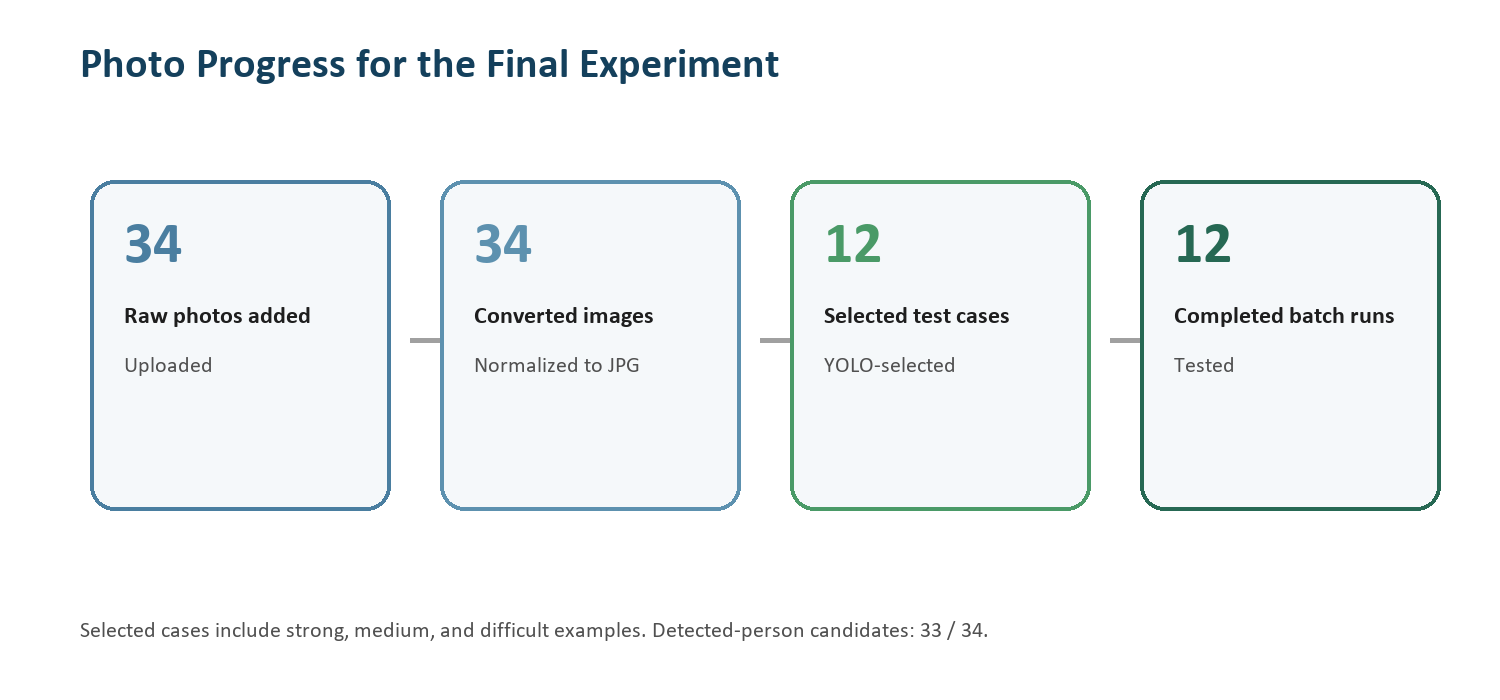
\includegraphics[width=\linewidth]{figures/photo_progress_card.png}}
\caption{Photo preparation progress. Thirty-four uploaded photos were converted and screened, and twelve images were selected for formal batch testing.}
\label{fig:progress}
\end{figure}

\subsection{YOLO-Guided SAM}
In the strongest version of the pipeline, YOLOv8n first detects the person bounding box. The detected box is expanded slightly and then used as a box prompt for SAM. This design reduces the ambiguity of automatic mask selection because SAM receives a target region instead of searching the entire image freely.

After SAM generates candidate masks, the system selects the best mask using SAM confidence and edge alignment as supporting information. This selected mask is then cleaned with connected-component filtering and morphological operations.

\subsection{Edge Alignment Score}
Because this project does not yet include manually labeled ground-truth masks, the experiment uses edge alignment as a proxy metric. First, a Canny edge map is generated from the original image. Then the predicted mask boundary is extracted by subtracting an eroded mask from a dilated mask. A small tolerance is allowed by dilating the Canny edge map with a $5 \times 5$ kernel. The score is defined as:

\begin{equation}
S(M,E) = \frac{|B(M) \cap D(E)|}{|B(M)|},
\end{equation}

where $M$ is the predicted mask, $B(M)$ is the mask boundary, $E$ is the Canny edge map, and $D(E)$ is the dilated edge map. A higher score means that more mask-boundary pixels are close to image edges.

This metric is useful for comparing boundary behavior inside this project, but it is not a replacement for IoU or Dice score. A high edge alignment score does not always mean that the whole person mask is correct, especially when background edges are strong.

\subsection{Edge Refinement and GrabCut}
The edge refinement module generates several candidate masks using morphological opening, closing, erosion, and dilation. Each candidate is accepted only if its area remains close to the original mask area. The candidate with the highest edge alignment score is selected.

GrabCut is then used as a post-processing step. The initial model mask is converted into a foreground-background initialization. To avoid destructive refinement, the implementation compares the refined edge score with the initial score and rejects the GrabCut result if the boundary quality decreases too much.

\section{Experimental Setup}
\subsection{Dataset}
The test data came from photos uploaded for the final project. The workflow started with 34 raw photos. After conversion and YOLO-based screening, 12 images were selected as the formal test set. The selected images include different backgrounds, poses, lighting conditions, and person sizes. This is a small test set, so the result should be treated as a preliminary course-project result rather than a general benchmark.

\subsection{Baseline and Proposed Method}
To avoid ambiguous comparison, this report defines one baseline method and one proposed final method before presenting the complete version list. The baseline is the strongest simple pipeline available before adding YOLO guidance. The proposed method is the final automatic pipeline selected after adding localization and boundary refinement. Table~\ref{tab:baseline_proposed} summarizes this definition.

\begin{table}[htbp]
\caption{Baseline and Proposed Method Definition}
\begin{center}
\begin{tabular}{|c|p{5.4cm}|}
\hline
\textbf{Method} & \textbf{Definition and Purpose} \\
\hline
Baseline v1 & Automatic SAM mask generation with Canny edge scoring and GrabCut. This represents the non-YOLO reference pipeline. \\
\hline
Proposed v6 & YOLO person detection is used to create a SAM box prompt. The resulting mask is refined by Canny-guided edge refinement and GrabCut. This is the final automatic method. \\
\hline
\end{tabular}
\label{tab:baseline_proposed}
\end{center}
\end{table}

\subsection{Models and Versions}
The implementation used SAM ViT-B as the segmentation backbone, YOLOv8n as the person detector, and YOLOv8n-Seg as the direct segmentation baseline. The tested versions are shown in Table~\ref{tab:versions}. Manual prompt versions were prepared but skipped in batch testing because they require user-provided boxes or points.

\begin{table}[htbp]
\caption{Experimental Versions}
\begin{center}
\begin{tabular}{|c|p{5.7cm}|c|}
\hline
\textbf{Version} & \textbf{Modules} & \textbf{Runs} \\
\hline
v1 & SAM auto + Canny score + GrabCut & 12 \\
\hline
v2 & SAM auto + Canny score + edge refine + GrabCut & 12 \\
\hline
v3 & Manual box or points + SAM + Canny + GrabCut & skipped \\
\hline
v4 & Manual box or points + SAM + Canny + edge refine & skipped \\
\hline
v5 & YOLO detection + SAM + Canny + GrabCut & 12 \\
\hline
v6 & YOLO detection + SAM + Canny + edge refine + GrabCut & 12 \\
\hline
v7 & YOLO-Seg direct mask + Canny + edge refine & 12 \\
\hline
v8 & YOLO-Seg direct mask + Canny + GrabCut & 12 \\
\hline
\end{tabular}
\label{tab:versions}
\end{center}
\end{table}

\section{Results}
Table~\ref{tab:results} shows the quantitative comparison. The baseline version v1 achieved a mean edge alignment score of 0.8708. The best final version was v6, which achieved a mean score of 0.8855. This is an absolute improvement of 0.0147 and a relative improvement of about 1.7\% over the baseline. The improvement is modest, but v6 also had a stronger minimum score than v5, which suggests better stability across the selected images.

\begin{table}[htbp]
\caption{Edge Alignment Results on Twelve Test Images}
\begin{center}
\begin{tabular}{|c|c|c|c|}
\hline
\textbf{Version} & \textbf{Mean} & \textbf{Min.} & \textbf{Max.} \\
\hline
v1 & 0.8708 & 0.6176 & 0.9695 \\
\hline
v2 & 0.8666 & 0.6714 & 0.9825 \\
\hline
v5 & 0.8422 & 0.2756 & 0.9827 \\
\hline
v6 & \textbf{0.8855} & \textbf{0.7518} & \textbf{0.9827} \\
\hline
v7 & 0.5768 & 0.3595 & 0.7151 \\
\hline
v8 & 0.7918 & 0.4671 & 0.8991 \\
\hline
\end{tabular}
\label{tab:results}
\end{center}
\end{table}

\begin{figure}[htbp]
\centerline{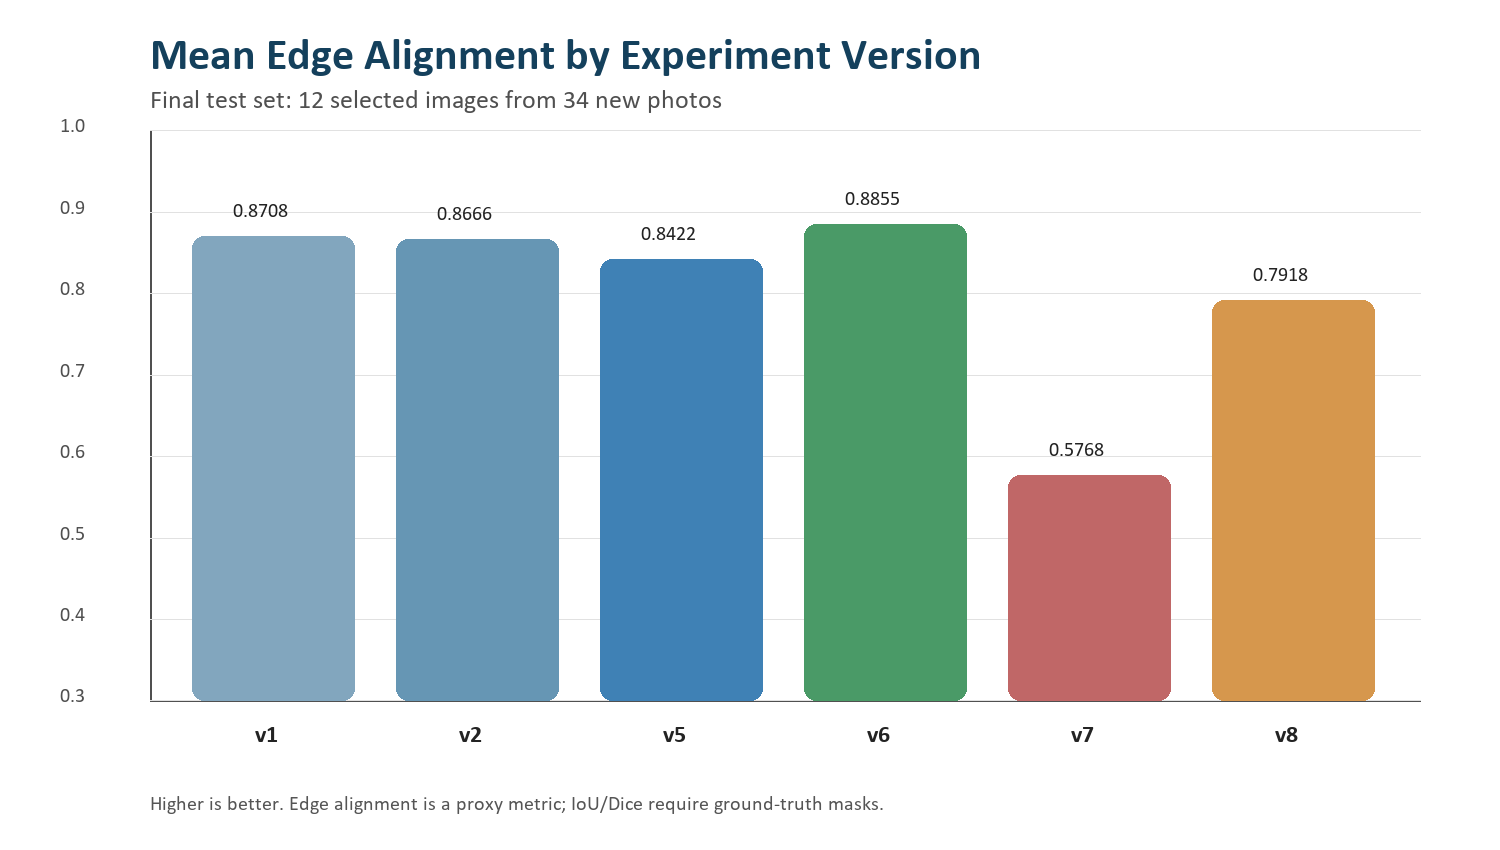
\includegraphics[width=\linewidth]{figures/final_version_bar_chart.png}}
\caption{Mean edge alignment comparison across tested versions. Version v6 achieved the highest average score in the selected test set.}
\label{fig:bar}
\end{figure}

The visual comparison in Fig.~\ref{fig:representative} shows a representative case where combining localization, segmentation, edge refinement, and GrabCut produces a cleaner person boundary. YOLO helps identify the target person area, SAM generates the main object mask, and refinement modules adjust the boundary using image edges and foreground-background separation.

\begin{figure}[htbp]
\centerline{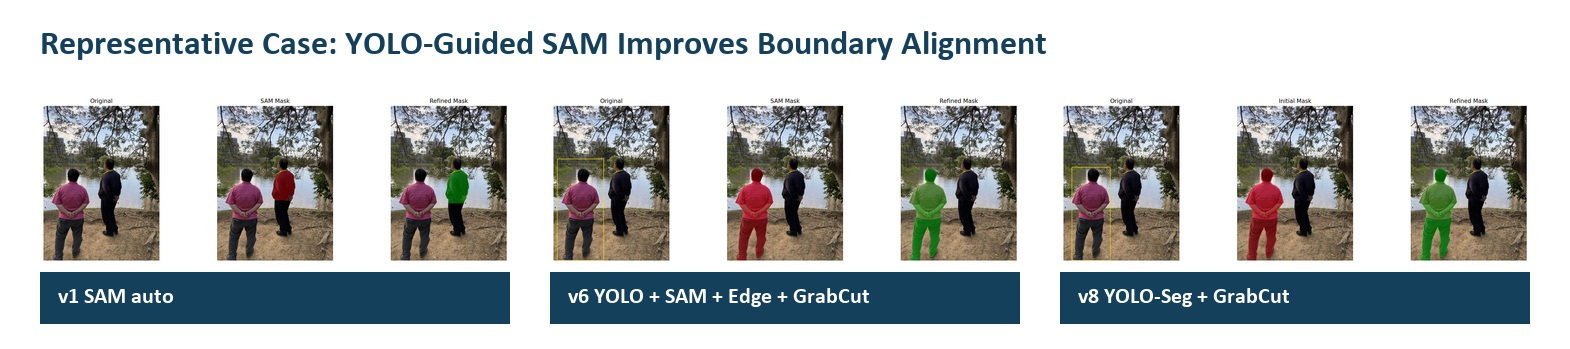
\includegraphics[width=\linewidth]{figures/representative_case_comparison.jpg}}
\caption{Representative comparison case. The multi-model pipeline improves the practical boundary quality compared with simpler outputs.}
\label{fig:representative}
\end{figure}

YOLO-Seg alone performed the weakest among the tested automatic versions, with a mean score of 0.5768. Adding GrabCut to YOLO-Seg improved the mean score to 0.7918, but it still remained below the SAM-based versions. This suggests that direct YOLO-Seg output is not enough for this dataset, but it can still provide useful initial masks for post-processing.

\section{Discussion}
The best result came from v6 because each module has a specific role. YOLO provides target localization, SAM generates a detailed segmentation mask from the detected box, edge refinement searches for a boundary that better matches local image edges, and GrabCut improves foreground-background separation. The combined design is more stable than using YOLO-Seg directly and slightly better than using automatic SAM with GrabCut.

However, the result should be interpreted carefully. Edge alignment measures how close the mask boundary is to Canny edges, not whether the entire person area is perfectly segmented. If the background has strong edges near the person, the score may be misleading. Also, without manual ground-truth masks, the experiment cannot report standard segmentation metrics such as Intersection over Union (IoU) or Dice score.

\subsection{Ground-Truth Evaluation Gap}
The current experiment intentionally does not report IoU or Dice score because no manually annotated binary masks were available. Reporting these metrics with model-generated masks as pseudo-ground truth would overstate the reliability of the result. Table~\ref{tab:metric_status} separates the reported metric from the metrics that require future annotation.

\begin{table}[htbp]
\caption{Metric Status and Evidence Level}
\begin{center}
\begin{tabular}{|c|c|p{3.2cm}|}
\hline
\textbf{Metric} & \textbf{Status} & \textbf{Reason} \\
\hline
Edge alignment & Reported & Computed from predicted mask boundaries and Canny edges. Useful for boundary consistency comparison. \\
\hline
IoU & Not reported & Requires manually labeled ground-truth masks. \\
\hline
Dice score & Not reported & Requires manually labeled ground-truth masks. \\
\hline
\end{tabular}
\label{tab:metric_status}
\end{center}
\end{table}

Fig.~\ref{fig:limitation} shows that failure cases can still occur when the subject boundary is visually ambiguous, when there are strong background edges, or when the person detection box does not fully represent the desired segmentation region.

\begin{figure}[htbp]
\centerline{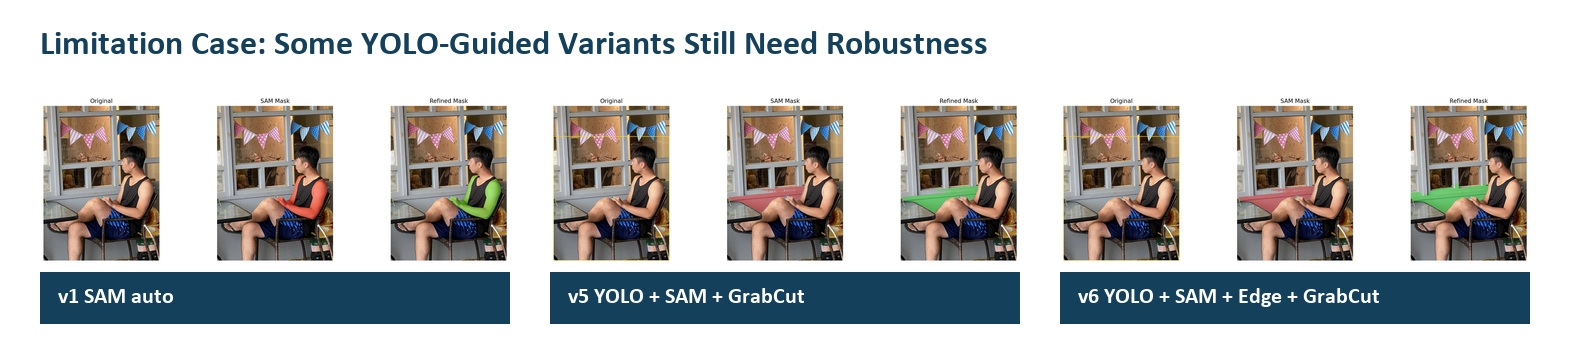
\includegraphics[width=\linewidth]{figures/limitation_case_comparison.jpg}}
\caption{Limitation case. The proposed pipeline improves several examples but can still fail under ambiguous boundaries or strong background edges.}
\label{fig:limitation}
\end{figure}

\section{Conclusion}
This project developed and tested a practical multi-model boundary refinement pipeline for person segmentation. The system combines YOLO detection, SAM segmentation, Canny edge-based boundary scoring, morphological edge refinement, and GrabCut foreground refinement. On twelve selected test images, the best version was YOLO-guided SAM with edge refinement and GrabCut, reaching a mean edge alignment score of 0.8855 compared with 0.8708 for the baseline.

The main conclusion is that using YOLO as an automatic box-prompt generator helps SAM focus on the intended person, and lightweight refinement modules can improve boundary stability. The improvement is modest and should be described as a preliminary improvement in edge alignment, not as a complete segmentation-accuracy claim. For future work, the project should add manually annotated ground-truth masks and evaluate IoU and Dice score. A larger test set with more difficult poses, occlusions, and backgrounds would also make the result more reliable.

\section*{Acknowledgment}
This work was completed as a final project for an Artificial Intelligence Applications course.

\begin{thebibliography}{00}
\bibitem{kirillov2023segmentanything}
A. Kirillov, E. Mintun, N. Ravi, H. Mao, C. Rolland, L. Gustafson, T. Xiao, S. Whitehead, A. C. Berg, W.-Y. Lo, P. Dollar, and R. Girshick, ``Segment anything,'' in \textit{Proc. IEEE/CVF Int. Conf. Computer Vision}, 2023, pp. 4015--4026.

\bibitem{gaus2024variationalprompting}
Y. F. A. Gaus, N. Bhowmik, B. K. S. Isaac-Medina, and T. P. Breckon, ``Performance evaluation of Segment Anything Model with variational prompting for application to non-visible spectrum imagery,'' \textit{arXiv preprint arXiv:2404.12285}, 2024.

\bibitem{mazurowski2023sammedical}
M. A. Mazurowski, H. Dong, H. Gu, J. Yang, N. Konz, and Y. Zhang, ``Segment Anything Model for medical image analysis: An experimental study,'' \textit{Medical Image Analysis}, p. 102918, 2023.

\bibitem{terven2023yoloreview}
J. Terven and D. Cordova-Esparza, ``A comprehensive review of YOLO architectures in computer vision: From YOLOv1 to YOLOv8 and YOLO-NAS,'' \textit{Machine Learning and Knowledge Extraction}, vol. 5, pp. 1680--1716, 2023.

\bibitem{canny1986computational}
J. Canny, ``A computational approach to edge detection,'' \textit{IEEE Transactions on Pattern Analysis and Machine Intelligence}, vol. PAMI-8, no. 6, pp. 679--698, 1986.

\bibitem{rother2004grabcut}
C. Rother, V. Kolmogorov, and A. Blake, ``GrabCut: Interactive foreground extraction using iterated graph cuts,'' \textit{ACM SIGGRAPH}, vol. 23, no. 3, pp. 309--314, 2004.
\end{thebibliography}

\end{document}
